\documentclass{amsart}

\usepackage{enumitem}
\usepackage{commath}
\usepackage{graphicx}

\title{Evaluation Questions for Scholarship Calculus}
\author{Alexander Elzenaar}

\begin{document}

\maketitle
\begin{abstract}
  The following are a set of questions suitable for evaluating possible scholarship calculus candidates; they require
  more creative thought than standard L2 questions, but should require no more technical knowledge than that learned
  in level two and below. The difficulty is generally increasing, but in no way are the questions ordered.
\end{abstract}

\begin{enumerate}\bfseries
  \item Convince me that $ 123^{-7} $ should be equal to $ \frac{1}{123^7} $. What if we adopt an alternative definition?
\end{enumerate}

Of course, here I am looking for the standard `each time we add one to the power we multiply by 123, so each time we subtract
one we must divide' answer (although other answers would be nice to see) --- the main thing I am actually looking for is an
understanding that negative powers are a \emph{convenient definition} rather than something which is forced upon us.

In terms of an alternative definition, one could (for example) define (for positive integer $ n $) $ x^{-n} $ to be equal to $ x^n $.
One immediate problem with this is that the product rule for powers no longer works --- if $ m $ is also positive, then $ x^m x^{-n} = x^m x^n = x^{m + n} $
rather than the $ x^{m - n} $ that is much more natural.

\filbreak\begin{enumerate}[resume]\bfseries
  \item How many (real) roots does $ -x^{1024} - x^{512} + 1 = 0 $ have?
\end{enumerate}

They should notice the function is a quadratic, use the discriminant of the quadratic to work out how many possible
values of $ x^{512} $ there are, and then notice that 512 is even so they need to double their answer.

\filbreak\begin{enumerate}[resume]\bfseries
  \item What is the largest rectangle you can fit inside a right-angled triangle?
\end{enumerate}

I am mainly looking to see that they recognise the applicability of calculus; do they draw a diagram? Are they communicating
well? The calculation itself should be fairly straightforward. The geometric possibility here is also interesting.

\filbreak\begin{enumerate}[resume]\bfseries
  \item Find a general formula for the sum of the first $ n $ natural numbers; i.e. find a simple formula that
        gives the same result as $ 1 + 2 + \cdots + n $.
\end{enumerate}

This question is normally quite successful (I have seen several pretty solutions from candidates), but I tend to no
longer use it as what I am looking for is a \emph{new} approach --- I think that at this stage I have seen every possible
way to prove the relevant result that one could come up with easily (the formula is $ n(n+1)/2 $). Several proofs
are outlined in my generic L3 maths notes, but that document does not include my favourite proof of this result (a geometric
proof involving counting dots).

\filbreak\begin{enumerate}[resume]\bfseries
  \item Explain to me why the sum of the first $ n $ odd numbers is simply $ n^2 $.
\end{enumerate}

In the same vein as the sum of the first $ n $ natural numbers; of course, this immediately suggests that the sum
of the first $ n $ even numbers is $ 2n(2n+1)/2 - n^2 = 2n^2 + n = n^2 + n $! Is there a nice geometric proof of this
like for the sum of odd numbers?

\filbreak\begin{enumerate}[resume]\bfseries
  \item Is $ \sqrt{7} $ a rational number?
  \item How many primes are there?
\end{enumerate}
I'm mainly looking for definitions; I am happy to guide candidates through the proofs (read: I expect to guide them).

\filbreak\begin{enumerate}[resume]\bfseries
  \item I've defined a function $ \sigma $ such that $ \sigma' = -\sigma $, and such that $ \sigma(3) = 3 $. What shape does the graph
        of $ \sigma $ have around 3?
\end{enumerate}

Here I'm looking for intuitive knowledge of derivatives and the shape of curves. Should be quite straightforward.

\filbreak\begin{enumerate}[resume]\bfseries
  \item Consider the series
        \begin{displaymath}
          \sum_{n = 1}^N \frac{1}{n(n + 1)}.
        \end{displaymath}
        Can you tell me its value when $ n = 1 $, $ n = 2 $, $ n = 5 $, $ n = 2017 $?
\end{enumerate}

Of course, this is a telescoping series (this can easily be seen by taking a partial fraction expansion). I would probably
not use sigma notation with the candidate (unless I was sure they had seen it before); I would expect to guide them through
using the partial fraction expansion and writing out the first few terms.

\filbreak\begin{enumerate}[resume]\bfseries
  \item Prove Thale's theorem: an angle inscribed in a semicircle is always right. Is the converse true?
\end{enumerate}

There is a very pretty proof of this (draw the other half of the rectangle); I have not tried this, students may just
try to use trigonometry (which works, of course) or have already seen the proof. I prefer to use statements with more nuance.

The converse \emph{is} true (a right triangle in a circle has a diameter for a base); again, draw the rectangle and notice that the centre of
the rectangle lies on the base and is equidistant from every corner.

\filbreak\begin{enumerate}[resume]\bfseries
  \item Explain to me the purpose of proof in mathematics.
  \item Which is more beautiful: the theorem or the definition?
\end{enumerate}

The first should be quite a nice discussion --- one hopes that students understand the question, of course. The second I am
not so sure of given the way mathematics is taught at colleges. I do like philosophical questions though. Rephrase?

\filbreak\begin{enumerate}[resume]\bfseries
  \item Are there more even numbers than natural numbers? Rational numbers than natural numbers? Real numbers than natural numbers?
\end{enumerate}

Here I am looking for a discussion of size of sets; whether or not they come up with Cantor's definition is irrelevant. Of course, we have obvious
bijections from $ \mathbb{N} $ to $ 2\mathbb{N} $ (the canonical bijection $ n \mapsto 2n $) and from $ \mathbb{N} $ to $ \mathbb{Q} $ (the zig-zag
bijection); then we have Cantor's proof that $ \abs{\mathbb{N}} \neq \abs{\mathbb{R}} $, which is not as obvious.

\filbreak\begin{enumerate}[resume]\bfseries
  \item Label the corners of a square $ \square $ as $ A $, $ B $, $ C $, and $ D $. Let us call a mapping $ \alpha : \square \to \square $ a \emph{symmetry}
        if it sends corners to corners (i.e. folding the square is not a symmetry). For example, any rotation or reflection is a symmetry. How many possible
        distinct symmetries are there? What is the minimum length of a list of symmetries we can write down such that any symmetry can be `generated' by performing
        symmetries on our list one after the other?
\end{enumerate}

Obviously we are describing the dihedral group $ D_8 $. There are eight symmetries (rotations by 0, 90, 180, and 270 degrees; and reflections
along both vertical and both diagonal axes) and two generators (the 90 degree rotation and any reflection):
\begin{center}
  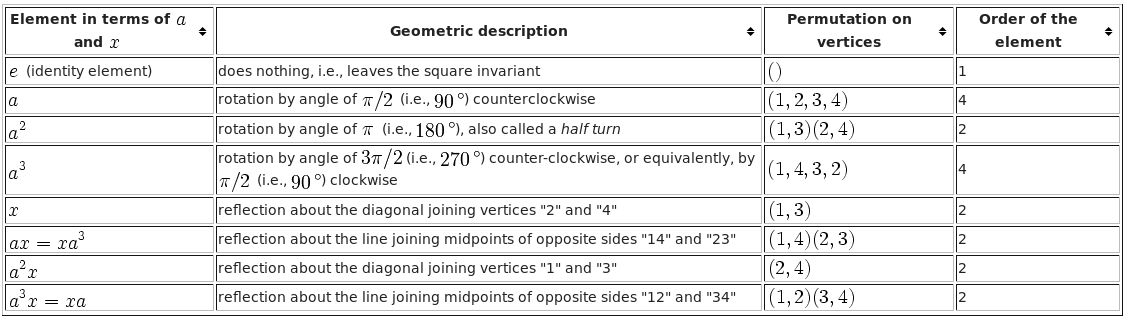
\includegraphics[width=\textwidth]{symmetriesofsquare}
\end{center}

\filbreak\begin{enumerate}[resume]\bfseries
  \item Consider the point $ P = (0, a) $ and the line $ d $ defined by $ y = -a $. Show that all the points $ (x, y) $ equidistant from the point and the
        line satisfy a quadratic equation. What about all the points such that the ratio of the distance from the point to $ P $ and $ (x,y) $ is $ e $,
        where $ 0 \leq e \leq \infty $?
\end{enumerate}

When in doubt, get them to derive an entire L3 standard by themselves. The parabola ($ e = 1 $) is straightforward, I have not tried circles, ellipses, and
hyperbolae myself but they can't be that hard.

\filbreak\begin{enumerate}[resume]\bfseries
  \item Show that for every natural number $ n > 1 $ there is some polynomial $ p(x) $ such that $ x^n - 1 = (x - 1)p(x) $.
\end{enumerate}
May be too technical.

\end{document}
